%% 
%% Copyright 2019-2024 Elsevier Ltd
%% 
%% Version 2.4
%% 
%% This file is part of the 'CAS Bundle'.
%% --------------------------------------
%% 
%% It may be distributed under the conditions of the LaTeX Project Public
%% License, either version 1.2 of this license or (at your option) any
%% later version.  The latest version of this license is in
%%    http://www.latex-project.org/lppl.txt
%% and version 1.2 or later is part of all distributions of LaTeX
%% version 1999/12/01 or later.
%% 
%% The list of all files belonging to the 'CAS Bundle' is
%% given in the file `manifest.txt'.
%% 
%% Template article for cas-sc documentclass for 
%% single column output.

\documentclass[a4paper,fleqn]{cas-sc}
\usepackage{placeins}
\usepackage[authoryear,longnamesfirst]{natbib}
\usepackage{amssymb}
\usepackage{blkarray}
\usepackage{amsmath}
\usepackage{float}
\usepackage{mathtools}
\usepackage{subfigure}
\usepackage{subcaption}
\usepackage{tikz}
\usetikzlibrary{arrows.meta}
\usetikzlibrary{positioning} 
\usepackage{amsthm}

\usepackage{ragged2e}
\usepackage{caption}
\usepackage[ruled,vlined]{algorithm2e}

%%%Author macros
\def\tsc#1{\csdef{#1}{\textsc{\lowercase{#1}}\xspace}}
\tsc{WGM}
\tsc{QE}
\tsc{EP}
\tsc{PMS}
\tsc{BEC}
\tsc{DE}
%%%
\newtheorem{thm}{Theorem}[section]
\newtheorem{asp}{Assumption}[section]
\newtheorem{lm}{Lemma}[section]
\newtheorem{prop}{Proposition}[section]
\newtheorem{deff}{Definition}[section]
\newtheorem{clm}{Claim}[section]
\newtheorem{cor}[thm]{Corollary}
\newtheorem{pron}[thm]{Proposition}
% \theoremstyle{definition}
\newtheorem{defn}[thm]{Definition}
\newtheorem{hyp}[thm]{Hypotheses}
% \theoremstyle{remark}
\newtheorem{remark}{Remark}[section]
\newtheorem{rem}{Remark}[section]
\newtheorem{exam}{Example}[section]
\numberwithin{equation}{section}
\newcommand{\weakto}{\mathrel{\rightharpoonup}}

% MATH -----------------------------------------------------------------
\DeclareMathOperator{\RE}{Re}
 \DeclareMathOperator{\IM}{Im}
\DeclareMathOperator{\ess}{ess}
\DeclareMathOperator{\inte}{int}
\DeclareMathOperator{\suppo}{supp}
\DeclareMathOperator{\trace}{tr}
\DeclareMathOperator{\sgn}{sgn}
\DeclareMathOperator{\LIM}{LIM}

\newcommand{\eps}{\varepsilon}
\newcommand{\To}{\longrightarrow}
\newcommand{\h}{\mathcal{H}}
\newcommand{\A}{\mathcal{A}}
\newcommand{\B}{\mathcal{B}}
\newcommand{\fB}{\mathfrak{B}}
\newcommand{\p}{\mathfrak{p}}
\newcommand{\m}{\mathfrak{m}}
\newcommand{\C}{\mathcal{C}}
\newcommand{\D}{\mathcal{D}}
\newcommand{\DD}{\mathbb{D}}
\newcommand{\UU}{\mathbb{U}}
\newcommand{\M}{\mathcal{M}}
\newcommand{\F}{\mathcal{F}}
\newcommand{\X}{\mathcal{X}}
\newcommand{\E}{\mathbb{E}}
\newcommand{\cv}{\mathbf{v}}
\newcommand{\bs}{\mathbf{s}}
\newcommand{\fE}{\mathfrak{E}}
\newcommand{\CE}{\mathcal{E}}
\newcommand{\Lom}{\mathcal{L}}
\newcommand{\BL}{\mathbb{L}}
\newcommand{\N}{{\mathbb{Z}}_+}
\newcommand{\Q}{{\mathbb{Q}}}
\newcommand{\Z}{\mathbb{Z}}
\newcommand{\W}{\mathfrak{H}}
\newcommand{\V}{\mathcal{V}}
\newcommand{\HB}{\mathbb{H}}
\newcommand{\K}{\mathcal{K}}
\newcommand{\BX}{\bar{X}}
\newcommand{\BY}{\bar{Y}}
\newcommand{\BS}{\mathbf{S}}
\newcommand{\BZ}{\mathbf{Z}}
\newcommand{\MCZ}{\{\BZ(kT),k\in\N\}}
\newcommand{\FU}{\mathfrak{U}}
\newcommand{\FUWP}{\mathfrak{U}(\{\wdt \Pi_{n}\})}
\newcommand{\FUP}{\mathfrak{U}(\{\wdt \Pi_{n_k}^{\bz_k}\})}
\newcommand{\PZ}{\mathcal{P}_{inv}(\R^{2}_+\times\M)}
\newcommand{\PPZ}{\mathcal{P}_{inv}(\partial\R^{2,\circ}_+\times\M)}
\newcommand{\PUB}{\mathcal{P}((0,\infty)\times[0,\infty)\times[0,M])}
\newcommand{\PP}{\mathbb{P}}
\newcommand{\BOP}{\mathbf{B}}
\newcommand{\BH}{\mathbf{B}(\mathcal{H})}
\newcommand{\KH}{\mathcal{K}(\mathcal{H})}
\newcommand{\R}{\mathbb{R}}
\newcommand{\Complex}{\mathbb{C}}
\newcommand{\BF}{\mathbb{F}}
\newcommand{\RPlus}{\Real^{+}}
\newcommand{\Polar}{\mathcal{P}_{\s}}
\newcommand{\Poly}{\mathcal{P}(E)}
\newcommand{\EssD}{\mathcal{D}}
\newcommand{\States}{\mathcal{T}}
\newcommand{\abs}[1]{\left\vert#1\right\vert}
\newcommand{\set}[1]{\left\{#1\right\}}
\newcommand{\seq}[1]{\left<#1\right>}
\newcommand{\norm}[1]{\left\Vwtrt#1\right\Vwtrt}
\newcommand{\essnorm}[1]{\norm{#1}_{\ess}}
\numberwithin{equation}{section}
\newcommand{\1}{\boldsymbol{1}}
\newcommand{\bbeta}{\boldsymbol{b }}
\newcommand{\0}{\boldsymbol{0}}
\newcommand{\blue}[1]{{\leavevmode\color{blue}#1}}
\newcommand{\red}[1]{{\leavevmode\color{red}[#1]}}

\newcommand{\wdt}{\widetilde}
\newcommand{\wdh}{\widehat}
\newcommand{\op}{{\mathcal L}}
\newcommand{\lbar}{\overline}
\newcommand{\bed}{\begin{equation}}
\newcommand{\eed}{\end{equation}}
\newcommand{\bea}{\bed\begin{array}{rl}}
\newcommand{\eea}{\end{array}\eed}
\newcommand{\ad}{&\!\!\!\disp}
\newcommand{\aad}{&\disp}
\newcommand{\barray}{\begin{array}{ll}}
\newcommand{\earray}{\end{array}}
\newcommand{\diag}{{\rm diag}}
\newcommand{\dist}{{\rm dist}}
\newcommand{\subscript}[2]{$#1 _ #2$}
\def\disp{\displaystyle}
\newcommand{\rr}{{\Bbb R}}

 \font\inh=cmr10 \font\cto=cmr10
\font\tit=cmbx12 \font\tmd=cmbx10 \font\ab=cmti9 \font\cn=cmr9
\def\ker{\text{Ker}}
\def\bar{\overline}
\def\hat{\widehat}
\def\a.s{\text{\;a.s.\;}}
\def\supp{\text{supp\,}}
\def\bnu{\boldsymbol{\nu}}
\def\bmu{\boldsymbol{\nu}}
\def\bdelta{\boldsymbol{\delta}}
\newcommand{\SZI}{\R^{2,\circ}_+\times\M}
\newcommand{\SZ}{\R^{2}_+\times\M}
\newcommand{\SZB}{\partial\R^{2}_+\times\M}
\newcommand{\Se}{\overline{\mathcal{S}}}
\newcommand{\Ve}{\overline{\mathcal{V}}}
\newcommand{\See}{\widetilde{S}^\theta}
\newcommand{\Swt}{\widetilde{S}^\theta}
\newcommand{\Vwt}{\widetilde{V}^\theta}
\newcommand{\wtau}{\widetilde\tau}
\newcommand{\bz}{\mathbf{z}}
\newcommand{\bp}{\mathbf{p}}
\newenvironment{eqcite}{
	\begin{equation}
		\begin{aligned}
		}{
		\end{aligned}
	\end{equation}}
\def\beq{\begin{eqcite}}
	
	\def\eeq{\end{eqcite}}

\usepackage{hyperref}
\newtheorem{theorem}{Theorem}[section] 
\newtheorem{lemma}[theorem]{Lemma}  
\newtheorem{proposition}[theorem]{Proposition}
\newtheorem{corollary}[theorem]{Corollary}

\makeatletter
\newcommand{\lemmaautorefname}{Lemma}
\newcommand{\propositionautorefname}{Proposition}
\newcommand{\corollaryautorefname}{Corollary}
\makeatother


\begin{document}

\let\WriteBookmarks\relax
\def\floatpagepagefraction{1}
\def\textpagefraction{.001}
\shorttitle{Optimal Insulin Therapy with Glucagon in Type 2 Diabetes}
\shortauthors{D.Q. Nguyen et al.}
%\begin{frontmatter}

\title [mode = title]{Optimal Insulin Therapy and the Importance of Glucagon in the Treatment of  Type 2 Diabetes: A Mathematical Modelling Approach}

\author[hus]{Dinh Quang Nguyen}
\ead{dinhquang120420041234@gmail.com}

\author[hus]{Anh Minh Tran}
\ead{anhminhtran.09.01.2003@gmail.com}

\author[hos]{Thuy Hang Nguyen}


\author[hus]{Trong Hieu Nguyen}
\cormark[1]
\ead{hieunguyentrong@gmail.com}


\affiliation[hus]{
    organization={University of Science, Vietnam National University},
    addressline={334 Nguyen Trai St, Thanh Xuan},
    city={Hanoi},
    country={Vietnam}
}

\affiliation[hos]{
    organization={Saint Paul General Hospital},
    addressline={12 Chu Van An St, Ba Dinh},
    city={Hanoi},
    country={Vietnam}
}

\cortext[cor1]{Corresponding author}

\begin{abstract}
In this study, we develop a system of nonlinear differential equations describing the glucose-insulin-glucagon dynamics to clarify the role of glucagon in the treatment of type 2 diabetes and to propose an optimal insulin injection strategy. The model incorporates key physiological feedback mechanisms governing glucose regulation and captures the interaction between hormonal responses and metabolic processes. We perform a qualitative analysis of the system, including the characterization of equilibrium states and their stability, to better understand the underlying dynamical behavior. In addition, two optimal control frameworks are introduced to determine insulin administration strategies that maintain glucose levels within a desired range while minimizing potential side effects. Numerical simulations are conducted to illustrate the theoretical findings and to highlight the impact of glucagon on treatment outcomes. The results suggest that incorporating glucagon dynamics can significantly influence the effectiveness of insulin therapy, providing useful insights for improving clinical management of type 2 diabetes.
\end{abstract}


\begin{keywords}
Impulsive differential equations \sep Optimal control \sep Type 2 Diabetes \sep Insulin \sep Glucagon
\end{keywords}

\makeatletter
\let\printorcid\relax
\makeatother

\maketitle

\section{Introduction}

\section{Mathematical model}
Let $G_1$ denote the carbohydrate intake per meal (g), $G_2$ the blood glucose concentration (mg/dL), $G$ the plasma glucagon concentration (pg/dL), and $I$ the plasma insulin concentration ($\mu$U/mL). All parameters are assumed to be positive for biological reasons, and the model is formulated as follows:
\begin{equation}
    \begin{cases}
        G_1' = -\alpha_1 G_1, \\
        G_2' = \alpha_2 G_1 - \beta I G_2 - \gamma G_2 + \eta G,\\
        G' = \sigma - z I G - dG, \\
        I' = \dfrac{\mu G_2^2}{K^2 + G_2^2} - nI.
    \end{cases}
    \label{eq: model with no treatment}
\end{equation}

%We propose a nonlinear dynamical framework that captures the essential regulatory mechanisms of glucose homeostasis in type 2 diabetes. The model combines exogenous input with endogenous hormonal feedback, leading to a coupled system in which glucose levels are controlled through competing production and utilization processes.

The first equation models the depletion of carbohydrates ingested per meal in the digestive system. The amount of carbohydrate. The amount of carbohydrates is converted into blood glucose through the term $\alpha_2 G_1$. A central feature of the model lies in the interaction between glucose and hormones. In particular, glucose dynamics are influenced by both uptake and production terms, as reflected in expressions of the form \( -\beta I G_2 \) and \( \eta G \), highlighting the opposing roles of insulin and glucagon \cite{SaltielKahn2001Insulin,UngerOrci1981Glucagon}. The parameter $\gamma$ represents the basal, insulin-independent glucose clearance rate, commonly referred to as glucose effectiveness, accounting for glucose uptake by insulin-independent tissues (e.g., brain and red blood cells) and renal excretion \cite{Bergman2021MinimalModelHistory}.
%Meanwhile, glucagon itself is subject to inhibition driven by insulin through a bilinear interaction term \( -z I G \), forming a negative feedback loop that stabilizes the system.
The third equation describes the variation of the plasma glucagon. We assume that the parameter $\sigma$ represents the basal glucagon production rate. The parameter $d$  represents the basal glucagon clearance rate, accounting for its degradation and removal from circulation primarily by renal metabolism \cite{Emmanouel1978GlucagonMetabolism}. An important term in this equation is $zIG$, representing insulin-mediated inhibition of glucagon secretion. This biologically important phenomenon has been reported in numerous experimental and physiological studies \cite{Kaneko1999PI3KGlucagon,Kawamori2009InsulinGlucagon,Vergari2019SGLT2Somatostatin}. The final equation describes plasma insulin dynamics. A key component is the nonlinear insulin response, modeled through Hill function of the form \(\frac{\mu G_2^2}{K^2 + G_2^2},\) which introduces a threshold effect in hormone secretion. The parameter $K$ represents the sensitivity constant controlling how strongly blood glucose stimulates insulin production, determining the saturation level of the insulin secretion response. This functional response is widely used in studies modeling insulin production in response to blood glucose \cite{Buchwald2011,Huang2012,Gallenberger2012,DAbbicco2016}. The formulation allows the model to reproduce realistic physiological behavior, including saturation at high glucose levels and reduced sensitivity at low concentrations. The parameter $n$ represents the rate of insulin clearance from the circulatory system.

%These coupled nonlinearities generate rich dynamical behavior, making the system suitable for capturing complex phenomena such as multiple steady states or transitions between glycemic regimes. Overall, the proposed model provides a mathematically tractable yet biologically meaningful framework for analyzing glucose-hormone interactions and for exploring optimal therapeutic strategies involving insulin and glucagon regulation.

\begin{table}[H]
    \centering
    \begin{tabular}{cp{9cm}cc}
        \hline
        \textbf{Symbol} & \textbf{Description} & \textbf{Unit} \\
        \hline
        $\alpha_1$ & Rate of carbohydrate absorption/decay from $G_1$ & 1/minute \\

        $\alpha_2$ & Conversion rate from ingested carbohydrate to blood glucose & [(mg/dL)/g]/minute \\

        $\beta$ & Insulin-dependent glucose uptake rate & (mL/\(\mu\)U)/minute \\

        $\gamma$ & Basal glucose clearance rate & 1/minute \\

        $\eta$ & Glucagon-induced glucose production rate & [(mg/dL)/(pg/mL)]/minute \\

        $\sigma$ & Basal glucagon secretion rate & (pg/mL)/minute \\

        $z$ & Insulin-mediated inhibition rate of glucagon & (mL/\(\mu\)U)/minute \\

        $d$ & Glucagon degradation rate & 1/minute \\

        $\mu$ & Maximum insulin secretion rate & (\(\mu\)U/mL)/minute \\

        $K$ & Half-saturation constant for glucose-stimulated insulin secretion & mg/dL \\

        $n$ & Insulin clearance rate & 1/minute \\
        \hline
    \end{tabular}
    \caption{Parameters used in the model and their descriptions.}
    \label{table:parameters}
\end{table}

\begin{table}
    \centering
    \begin{tabular}{clcc}
        \hline
        \textbf{Variable} & \textbf{Description} & \textbf{Unit} \\
        \hline
        $G_1$ & Carbohydrate intake per meal & gram (g) \\ 
        $G_2$ & Blood glucose concentration & milligram per deciliter (mg/dL)\\
        $G$ & Glucagon concentration & picogram per deciliter (pg/dL) \\
        $I$ & Insulin concentration & micro-unit per milliliter (\(\mu\)U/mL) \\
        \hline
    \end{tabular}
    \caption{Variables used in the models.}
    \label{table: variables}
\end{table}

\begin{figure}
    \centering
    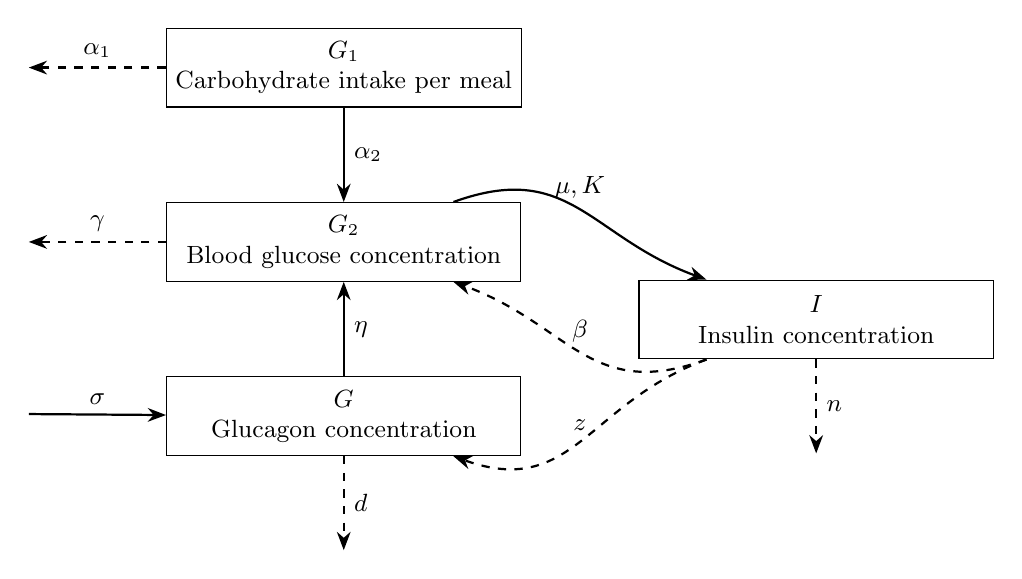
\begin{tikzpicture}[
    node distance=1.2cm and 2.4cm,
    box/.style={rectangle, draw, minimum width=4.5cm, minimum height=1cm, align=center},
    arrow/.style={-{Stealth}, thick},
    inhib/.style={-{Stealth}, thick, dashed},
    curved/.style={out=20,in=160, looseness=1.2},
    curvedback/.style={out=200,in=340, looseness=1.2},
    loop/.style={->, thick, looseness=3, min distance=6mm},
    every node/.style={font=\small}
    ]

    % Nodes
    \node[box] (G1) {$G_1$\\Carbohydrate intake per meal};
    \node[box, below=of G1] (G2) {$G_2$\\Blood glucose concentration};
    \node[box, below=of G2] (G) {$G$\\Glucagon concentration};
    \node[box] (I) at (6, -3.2) {$I$\\Insulin concentration};


    \draw[inhib] (G1) -- ++(-4cm, 0) node[midway, above] {$\alpha_1$};

    \draw[arrow] (G1) -- (G2) node[midway, right] {$\alpha_2$};

    \draw[inhib] (G2) -- ++(-4cm, 0) node[midway, above] {$\gamma$};

    \draw[arrow] (G) -- (G2) node[midway, right] {$\eta$};

    % \draw[loop, looseness=8] (G) to[out=150,in=210] node[left] {$\sigma$} (G);

    \draw[arrow] (-4, -4.4) -- (G) node[midway, above] {$\sigma$};

    \draw[inhib] (G) -- ++(0, -1.7cm) node[midway, right] {$d$};

    \draw[inhib] (I) -- ++(0, -1.7cm) node[midway, right] {$n$};

    \draw[arrow] (G2) to[curved] node[above] {$\mu, K$} (I);

    \draw[inhib] (I) to[curvedback] node[above] {$\beta$} (G2);
    
    \draw[inhib] (I) to[curvedback] node[above] {$z$} (G);
    
    \end{tikzpicture}

    \caption{Interaction between variables of the proposed model}
    \label{model}
\end{figure}

The system \eqref{eq: model with no treatment} satisfies the uniqueness of local solutions for each initial condition in $\mathbb{R}^4$ due to the vector field $F \in C^1(\mathbb{R}^4)$, where
\[
F(G_1, G_2, G, I) = \begin{pmatrix}
    -\alpha_1 G_1 \\
    \alpha_2 G_1 - \beta I G_2 - \gamma G_2 + \eta G\\
    \sigma - z I G - dG\\
    \dfrac{\mu G_2^2}{K^2 + G_2^2} - nI
\end{pmatrix}.
\]

\begin{proposition}
    The domain $\mathbb{R}^4_{\geq 0}$ is positively invariant for the system \eqref{eq: model with no treatment}. Furthermore, for any initial condition in $\mathbb{R}^4_{\geq 0}$, the solution of the system \eqref{eq: model with no treatment} is bounded and satisfies:
    \begin{enumerate}
        \item $\displaystyle\lim_{t \to +\infty} G_1 = 0,$
        \item $\displaystyle \frac{\eta \sigma}{\left(\beta\nu + \gamma\right)\left(z\nu + d\right)} \leq \underset{t \to +\infty}{\lim \inf} G_2 \leq \underset{t \to +\infty}{\lim \sup} G_2 \leq \frac{n\sigma}{\gamma d},$
        \item $\displaystyle \frac{\sigma}{z\nu + d}\leq \underset{t \to +\infty}{\lim \inf} G \leq \underset{t \to +\infty}{\lim \sup} G \leq \frac{\sigma}{d},$
        \item $\displaystyle \frac{\nu \kappa^2}{K^2 + \kappa^2}\leq \underset{t \to +\infty}{\lim \inf} I \leq \underset{t \to +\infty}{\lim \sup} I \leq \frac{\mu}{n},$
    \end{enumerate}
    where $\nu = \dfrac{\mu}{n}, \kappa = \dfrac{\eta \sigma}{\left(\beta\nu + \gamma\right)\left(z\nu + d\right)}.$
    Consequently, every solution of \eqref{eq: model with no treatment} is defined for all $t \geq 0$.
\end{proposition}

\begin{proof}
    Let the vector field $F = (f_1,f_2,f_3,f_4)$, where $f_i: \mathbb{R}^4_{\geq 0} \to \mathbb{R}, \; i =1,2,3,4$. Note that
    \[
        f_1(0,G_2,G,I) = 0, \quad  f_2(G_1,0,G,I) \geq 0, \quad f_3(G_1,G_2,0,I) > 0, \quad f_4(G_1,G_2,G,0) \geq 0. \\
    \]
    Hence, we conclude that the domain $\mathbb{R}^4_{\geq 0}$ is positively invariant for the system \eqref{eq: model with no treatment}.

    We now show the boundedness of $(G_1, G_2, G, I)$. 
    
    It is clear that $\displaystyle\lim_{t \to +\infty} G_1(t) = 0$. Since all state variables are non-negative, the dynamics of $G$ and $I$ satisfy $G' \leq \sigma - dG$ and $I' \leq \mu - nI$. Integrating these upper bounds gives $G(t) \leq G(0)e^{-dt} + \frac{\sigma}{d}(1 - e^{-dt})$ and $I(t) \leq I(0)e^{-nt} + \frac{\mu}{n}(1 - e^{-nt})$. As $t \text{ approaches } +\infty$, the superior limits are bounded by:
    \[
        \limsup_{t \to +\infty} G(t) \leq \frac{\sigma}{d} \quad \text{and} \quad \limsup_{t \to +\infty} I(t) \leq \frac{\mu}{n} = \nu.
    \]
    
    Consequently, for any arbitrary $\varepsilon > 0$, there exists a sufficiently large $T_\varepsilon > 0$ such that for all $t > T_\varepsilon$, $G_1(t) < \varepsilon$, $G(t) < \frac{\sigma}{d} + \varepsilon$, and $I(t) < \nu + \varepsilon$. Discarding the non-positive term $-\beta I G_2$, the equation for $G_2$ for $t > T_\varepsilon$ yields $G_2' \leq \alpha_2 \varepsilon - \gamma G_2 + \eta \left( \frac{\sigma}{d} + \varepsilon \right)$. The solution to this differential inequality satisfies:
    \[
        G_2(t) \leq G_2(T_\varepsilon)e^{-\gamma(t-T_\varepsilon)} + \frac{1}{\gamma}\left[\alpha_2 \varepsilon + \eta \left( \frac{\sigma}{d} + \varepsilon \right)\right]\left(1 - e^{-\gamma(t-T_\varepsilon)}\right).
    \]
    Passing to the limit as $t \text{ approaches } +\infty$ and subsequently as $\varepsilon \text{ approaches } 0$ establishes:
    \[
        \limsup_{t \to +\infty} G_2(t) \leq \frac{\eta\sigma}{\gamma d}.
    \]
    
    To establish the lower bounds, we utilize the obtained asymptotic limits. From $I(t) < \nu + \varepsilon$ for $t > T_\varepsilon$, the $G$ equation implies $G' \geq \sigma - (z(\nu + \varepsilon) + d)G$. Evaluating this expression leads to:
    \[
        G(t) \geq G(T_\varepsilon)e^{-(z(\nu + \varepsilon) + d)(t-T_\varepsilon)} + \frac{\sigma}{z(\nu + \varepsilon) + d}\left(1 - e^{-(z(\nu + \varepsilon) + d)(t-T_\varepsilon)}\right).
    \]
    
    Extracting the inferior limit as $t \text{ approaches } +\infty$ and subsequently as $\varepsilon \text{ approaches } 0$ provides:
    \[
        \liminf_{t \to +\infty} G(t) \geq \frac{\sigma}{z\nu+d}.
    \]
    
    By increasing $T_\varepsilon$ if necessary, we can assume that for all $t > T_\varepsilon$, $G(t) > \frac{\sigma}{z\nu+d} - \varepsilon$ also holds. Substituting this and $I(t) < \nu + \varepsilon$ into the $G_2$ dynamics gives $G_2' \geq \eta \left( \frac{\sigma}{z\nu+d} - \varepsilon \right) - (\beta(\nu + \varepsilon) + \gamma)G_2$. By integrating this relationship, we find:
    \[
        G_2(t) \geq G_2(T_\varepsilon)e^{-(\beta(\nu + \varepsilon) + \gamma)(t-T_\varepsilon)} + \frac{\eta \left( \frac{\sigma}{z\nu+d} - \varepsilon \right)}{\beta(\nu + \varepsilon) + \gamma}\left(1 - e^{-(\beta(\nu + \varepsilon) + \gamma)(t-T_\varepsilon)}\right).
    \]
    As $t \text{ approaches } +\infty$ and $\varepsilon \text{ approaches } 0$, we deduce:
    \[
        \liminf_{t \to +\infty} G_2(t) \geq \frac{\eta\sigma}{(\beta \nu + \gamma)(z\nu + d)} = \kappa.
    \]
    
    Finally, the function $f(x) = \frac{\mu x^2}{K^2+x^2}$ is strictly increasing for $x \geq 0$. Assuming $T_\varepsilon$ is large enough such that $G_2(t) > \kappa - \varepsilon$ for all $t > T_\varepsilon$, the dynamics of $I$ satisfy $I' \geq \frac{\mu(\kappa-\varepsilon)^2}{K^2+(\kappa-\varepsilon)^2} - nI$. Deriving the bound from this relation results in:
    \[
        I(t) \geq I(T_\varepsilon)e^{-n(t-T_\varepsilon)} + \frac{\mu(\kappa-\varepsilon)^2}{n(K^2+(\kappa-\varepsilon)^2)}\left(1 - e^{-n(t-T_\varepsilon)}\right).
    \]
    Evaluating the asymptotic behavior as $t \text{ approaches } +\infty$ and as $\varepsilon \text{ approaches } 0$ confirms:
    \[
        \liminf_{t \to +\infty} I(t) \geq \frac{1}{n} \frac{\mu\kappa^2}{K^2+\kappa^2} = \frac{\nu\kappa^2}{K^2+\kappa^2}.
    \]
\end{proof}

\begin{theorem}
The system \eqref{eq: model with no treatment} admits a unique positive equilibrium $E^*$, which is locally asymptotically stable.
\end{theorem}
\begin{proof}
To identify the equilibrium of the model, we examine the states at which the system remains unchanged over time. An equilibrium \((G_1^*,G_2^*, G^*, I^*)\) of \eqref{eq: model with no treatment} is defined as a solution of the algebraic system obtained by setting all time derivatives equal to zero, which can be expressed as
\[
    \begin{cases}
        0 = -\alpha_1 G_1^*, \\
        0 = \alpha_2 G_1^* - \beta I^* G_2^* - \gamma G_2^* + \eta G^*,\\
        0 = \sigma - z I^* G^* - dG^*, \\
        0 = \dfrac{\mu G_2^{*2}}{K^2 + G_2^{*2}} - nI^*.
    \end{cases}
\]

It is readily observed that \(G_1^* = 0\). From the second and third equations, one can express \(G_2^*\) and \(G^*\) explicitly in terms of \(I^*\) as follows:
\[
\begin{cases}
    G_2^*= \dfrac{\eta\sigma}{(\beta I^* +\gamma)(zI^*+d)},\\
    G^*= \dfrac{\sigma}{zI^*+d}.
\end{cases}
\]

Substituting the expression of \(G_2^*\) into the fourth equation yields
\[
\dfrac{\mu \left(\dfrac{\eta\sigma}{(\beta I^* +\gamma)(zI^*+d)}\right)^2}{K^2 + \left(\dfrac{\eta\sigma}{(\beta I^* +\gamma)(zI^*+d)}\right)^2} - nI^* =0,
\]
this equation can be rewritten as following
% \[
%     \varphi(I^*) := C_5 I^{*5} + C_4 I^{*4} + C_3 I^{*3} + C_2 I^{*2} + C_1 I^* - C_0 = 0,
% \]
\[
nI^*\left(K^2(\beta I^* +\gamma)^2(zI^*+d)^2 +\eta^2 \sigma^2\right) = \mu\eta^2\sigma^2.
\]

We define
\[
\varphi(I) = nI\left(K^2(\beta I +\gamma)^2(zI+d)^2 +\eta^2 \sigma^2\right).
\]
% where
% \[
% \begin{cases}
%     C_5 = K^2 z^2 \beta^2, \\
%     C_4 = K^2 \left(2z^2 \beta \gamma + 2zd \beta^2 \right), \\ 
%     C_3 = K^2 \left(z^2 \gamma^2 + 4zd \beta \gamma + d^2 \beta^2 \right), \\
%     C_2 = K^2 \left(2zd \gamma^2 + 2d^2 \beta \gamma \right), \\
%     C_1 = K^2 d^2 \gamma^2 + \eta^2 \sigma^2, \\
%     C_0 = -\dfrac{\mu}{n} \eta^2 \sigma^2.
% \end{cases}
% \]

It is straightforward to verify that \(\varphi'(I) \geq 0\) for all \(I \geq 0\), hence \(\varphi\) is strictly increasing on \([0,+\infty)\). Furthermore,
\[
\varphi(0)=0 < \mu\eta^2\sigma^2, \quad \lim_{I\to+\infty}\varphi(I)=+\infty.
\]

Therefore, by the Intermediate Value Theorem, the equation \(\varphi(I)=\mu\eta^2\sigma^2\) admits a unique positive solution \(I^*\). Consequently, the system admits a unique positive equilibrium
\[
E^* = \left(0, \dfrac{\eta\sigma}{(\beta I^* +\gamma)(zI^*+d)}, \dfrac{\sigma}{zI^*+d}, I^*\right).
\]

The Jacobian matrix at the equilibrium $E^*$ is given by
\[
J(E^*) =
\begin{pmatrix}
-\alpha_1 & 0 & 0 & 0 \\[6pt]
\alpha_2 & -\beta I^* - \gamma & \eta & -\beta G_2^* \\[6pt]
0 & 0 & -zI^* - d & -zG^* \\[6pt]
0 & \dfrac{2\mu K^2 G_2^*}{\left(K^2 + G_2^{*2}\right)^2} & 0 & -n
\end{pmatrix}.
\]

It is clear that the matrix is block lower triangular. Hence, one eigenvalue is immediately obtained as
\[
\lambda_1 = -\alpha_1 < 0.
\]

The remaining eigenvalues are determined by the $3 \times 3$ submatrix
\[
J_{G_2,G,I}(E_1^*) =
\begin{pmatrix}
-\beta I^* - \gamma & \eta & -\beta G_2^* \\[6pt]
0 & -zI^* - d & -zG^* \\[6pt]
\dfrac{2\mu K^2 G_2^*}{\left(K^2 + G_2^{*2}\right)^2} & 0 & -n
\end{pmatrix}.
\]

The trace of $J_{G_2,G,I}(E_1^*)$ is
\[
\mathrm{tr}(J_{G_2,G,I}(E_1^*))
= -(\beta I^* + \gamma) - (zI^* + d) - n.
\]

The determinant of $J_{G_2,G,I}(E_1^*)$ is 
\[
\det(J_{G_2,G,I}(E_1^*))
= -
(\beta I^* + \gamma)(zI^* + d)n - \frac{2\eta z \mu K^2 G^* G_2^*}{(K^2 + G_2^{*2})^2} - \frac{2\beta \mu K^2 G_2^{*2} (zI^* + d)}{(K^2 + G_2^{*2})^2}.
\]

Let $\psi(J_{G_2,G,I}(E_1^*))$ denote the sum of all principal minors of order two of $J_{G_2,G,I}(E_1^*)$. Then,
\[
\psi(J_{G_2,G,I}(E_1^*)) = (\beta I^* + \gamma)(zI^* + d) + n(\beta I^* + \gamma)
+ \frac{2\mu \beta K^2 G_2^{*2}}{(K^2 + G_2^{*2})^2} + n(zI^* + d).
\]

Since 
\[
\begin{cases}
    - \mathrm{tr}(J_{G_2,G,I}(E_1^*)) > 0, \\
    - \mathrm{det}(J_{G_2,G,I}(E_1^*)) > 0, \\
    \psi (J_{G_2,G,I}(E_1^*)) > 0,
\end{cases}
\]
therefore, to apply the Routh-Hurwitz criterion \cite{Hsu2013}, we consider the quantity
\[
\begin{aligned}
&-\mathrm{tr}(J_{G_2,G,I}(E_1^*)) \cdot \psi(J_{G_2,G,I}(E_1^*))
- \big(-\det(J_{G_2,G,I}(E_1^*))\big)\\
&= (\beta I^*+\gamma)^2(zI^*+d)
+ (\beta I^*+\gamma)(zI^*+d)^2 + n\left[(\beta I^*+\gamma) + (zI^*+d)\right]^2 + n^2\left[(\beta I^*+\gamma)+ (zI^*+d)\right] \\
&\quad + \frac{2\beta \mu K^2 (G_2^*)^2}{\left(K^2 + G_2^{*2}\right)^2}
\left[(\beta I^*+\gamma)+n\right] - \frac{2\eta z \mu K^2 G^* G_2^*}{\left(K^2 + G_2^{*2}\right)^2}\\
&= (\beta I^*+\gamma)^2(zI^*+d)
+ (\beta I^*+\gamma)(zI^*+d)^2 + n\left[(\beta I^*+\gamma) + (zI^*+d)\right]^2 + n^2\left[(\beta I^*+\gamma)+ (zI^*+d)\right] \\
&\quad + \frac{2\beta \mu K^2 (G_2^*)^2}{\left(K^2 + G_2^{*2}\right)^2}
\left[(\beta I^*+\gamma)+n\right] - \frac{2 z \mu K^2 G_2^{*2}}{\left(K^2 + G_2^{*2}\right)^2}\left(\beta I^* + \gamma\right)\\
&= (\beta I^*+\gamma)^2(zI^*+d)
+ (\beta I^*+\gamma)(zI^*+d)^2 + n\left[(\beta I^*+\gamma) + (zI^*+d)\right]^2 + n^2\left[(\beta I^*+\gamma)+ (zI^*+d)\right] \\
&\quad + \frac{2\beta \mu K^2 (G_2^*)^2}{\left(K^2 + G_2^{*2}\right)^2}
\left[(\beta I^*+\gamma)+n\right] - 2z\left(\beta I^* + \gamma\right)\frac{\mu G_2^{*2}}{K^2 + G_2^{*2}} \left(1 - \frac{G_2^{*2}}{K^2 + G_2^{*2}}\right) \\
&= (\beta I^*+\gamma)^2(zI^*+d)
+ (\beta I^*+\gamma)(zI^*+d)^2 + n\left[(\beta I^*+\gamma) + (zI^*+d)\right]^2 + n^2\left[(\beta I^*+\gamma)+ (zI^*+d)\right] \\
&\quad + \frac{2\beta \mu K^2 (G_2^*)^2}{\left(K^2 + G_2^{*2}\right)^2}
\left[(\beta I^*+\gamma)+n\right] - 2z\left(\beta I^* + \gamma\right)nI^* \left(1 - \frac{nI^*}{\mu}\right)\\
&= (\beta I^*+\gamma)^2(zI^*+d)
+ (\beta I^*+\gamma)(zI^*+d)^2 + n\left[(\beta I^*+\gamma)^2 + z^2I^{*2}+d^2 + 2d(\beta I^*+\gamma) + 2dzI^*)\right] \\
&\quad + n^2\left[(\beta I^*+\gamma)+ (zI^*+d)\right] + \frac{2\beta \mu K^2 (G_2^*)^2}{\left(K^2 + G_2^{*2}\right)^2}
\left[(\beta I^*+\gamma)+n\right] + 2z\left(\beta I^* + \gamma\right)\frac{nI^{*2}}{\mu} > 0.\\
\end{aligned}
\]

Hence, all eigenvalues of the submatrix \(J_{G_2,G,I}(E^*)\) have negative real parts. Together with \(\lambda_1 = -\alpha_1 < 0\), it follows that all eigenvalues of the Jacobian matrix \(J(E^*)\) have negative real parts. Therefore, the equilibrium \(E^*\) is always locally asymptotically stable.
\end{proof}

\section{Parameter Estimation}
The purpose of this section is to fit model \eqref{eq: model with no treatment} to the actual data. Notably, each parameter value is estimated from the data of each individual patient, allowing the parameter values to capture the individual biological characteristics of each patient. The data used were taken from \cite{Hall2018Glucotypes}. The dataset comprises glucose concentrations recorded at 5-minute intervals using continuous glucose monitoring (CGM) over a 3-hour period, spanning from 30 minutes before meal intake to 2.5 hours after the meal. In addition, nutritional information for each meal is provided (see \cite{Hall2018Glucotypes} for further details).  Therefore, no measurements of plasma glucagon and insulin are available over the observation period. Consequently, estimating the initial plasma concentrations of glucagon and insulin is essential for parameter estimation.

Inverse problems aim to combine mathematical models with observational data and arise in many areas of science and engineering. The solvability of such a task is usually classified through its well-posedness. A problem is well-posed if it has a unique solution that depends continuously on input or data. However, inverse problems are usually ill-posed in practice \cite{Latz2023BayesianWellPosed}. In particular, parameter estimation for ordinary differential equation (ODE) systems constitutes an inherently ill-posed inverse problem, especially in the context of experimental biological data. Such problems are characterized by several major challenges such as a non-convex optimization problem with multiple local minima, which is highly sensitive to initial guesses and measurement noise. As a consequence, optimization procedures are prone to convergence to local minima that may lack physiological interpretability.

A fundamental challenge arises from issues of parameter identifiability. In many biological models, parameters cannot be uniquely determined from the available observations, even under ideal noise-free conditions. This limitation becomes significantly more pronounced when the data are incomplete in our case, leading to situations in which multiple distinct parameter sets yield comparably good fits to the observed data.

To address this challange, we employ the two-stage procedure. First, we define a simple loss function as follows:
    \[
    \mathcal{L} (p) = \displaystyle\sum_{i=1}^N \left(G_2(t_i,p) - G_2^{\text{obs}}(t_i)\right)^2,
    \]
where $p = [\alpha_1, \alpha_2, \beta, \gamma, \eta, \sigma, z, d, \mu, n, K, G_0, I_0]$. The procedure of parameter estimation is divided into two steps, where the first stage finds a suitable initial guess $p_0$ and the second stage applies a local, fast-converging optimization to obtain $p$ based on $p_0$. 

More specifically, in the first stage, we employ the particle swarm optimization (PSO) \cite{Gad2022PSOReview}. This algorithm is a method that does not require gradient information and is capable of exploring the parameter space to approach a good global solution. However, it can be computationally expensive, as each particle must evaluate the loss function at every iteration; in parameter estimation for ODEs, this typically requires repeatedly solving ODEs, leading to a high overall computational cost. Therefore, in the first stage, the PSO algorithm is configured with a swarm size of 50 and a maximum of 50 iterations to identify a promising region in the parameter space. In the second stage, we employ the \textit{fmincon} function in MATLAB \cite{Lopez2014MATLABOptimization} with the initial
point $p_0$ obtained from the first stage. Furthermore, to eliminate physiologically unrealistic parameter values and reduce the occurrence of local minima, we propose the predicted parameter value ranges as presented in Table~\ref{table: range}. Parameter ranges were initially referenced from the literature \cite{GallardoHernandez2022MinimalModel,Kelly2019GlucagonModel} and subsequently refined to be suitable with the proposed model.

In our experiments, we estimate the parameters for two cases: a healthy individual and a diabetic individual. We then compare the corresponding parameter sets to investigate how physiological differences between the two cases are reflected in the estimated parameters, thereby providing biological insights into the pathological characteristics of type 2 diabetes. The estimated parameter values are presented in Table~\ref{table: parameter}.

\begin{table}[H]
\centering
\begin{tabular}{ccc}
\hline
\textbf{Parameter} & \textbf{Range} & \textbf{Reference} \\
\hline
$\alpha_1$ & $[0.004,\; 0.06]$ & Assume \\
$\alpha_2$ & $[8\times 10^{-5},\; 0.012]$ & Assume \\
$\beta$    & $[8\times 10^{-6},\; 0.006]$ & \cite{GallardoHernandez2022MinimalModel,Kelly2019GlucagonModel} \\
$\gamma$   & $[0.004,\; 0.06]$ & \cite{GallardoHernandez2022MinimalModel} \\
$\eta$     & $[8\times 10^{-6},\; 0.012]$ & Assume \\
$\sigma$   & $[0.4,\; 12]$ & Assume \\
$z$        & $[8\times 10^{-6},\; 0.012]$ & Assume \\
$d$        & $[0.008,\; 0.12]$ & \cite{Kelly2019GlucagonModel} \\
$\mu$      & $[0.08,\; 12]$ & Assume \\
$n$        & $[0.008,\; 0.6]$ & \cite{GallardoHernandez2022MinimalModel} \\
$K$        & $[75,\; 160]$ & Assume \\
$G_0$      & $[45,\; 125]$ & \cite{Kelly2019GlucagonModel} \\
$I_0$      & $[1.5,\; 30]$ & \cite{GallardoHernandez2022MinimalModel} \\
\hline
\end{tabular}
\caption{The predicted parameter value ranges used for model.}
\label{table: range}
\end{table}

\begin{figure}[H]
    \centering
    \begin{minipage}{0.48\textwidth}
        \centering
        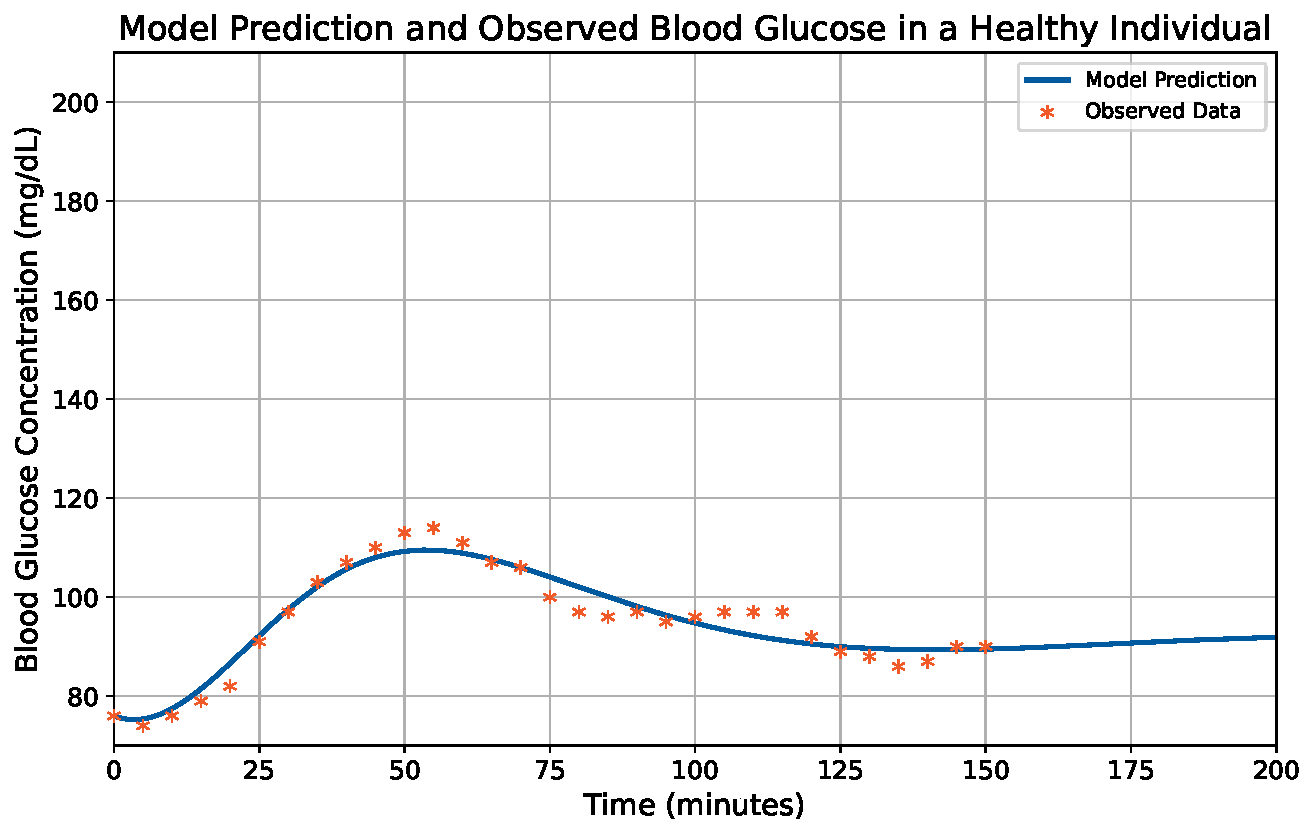
\includegraphics[width=\linewidth]{Figures/Model Prediction and Observed Blood Glucose in a Healthy Individual.pdf}
    \end{minipage}
    \hfill
    \begin{minipage}{0.48\textwidth}
        \centering
        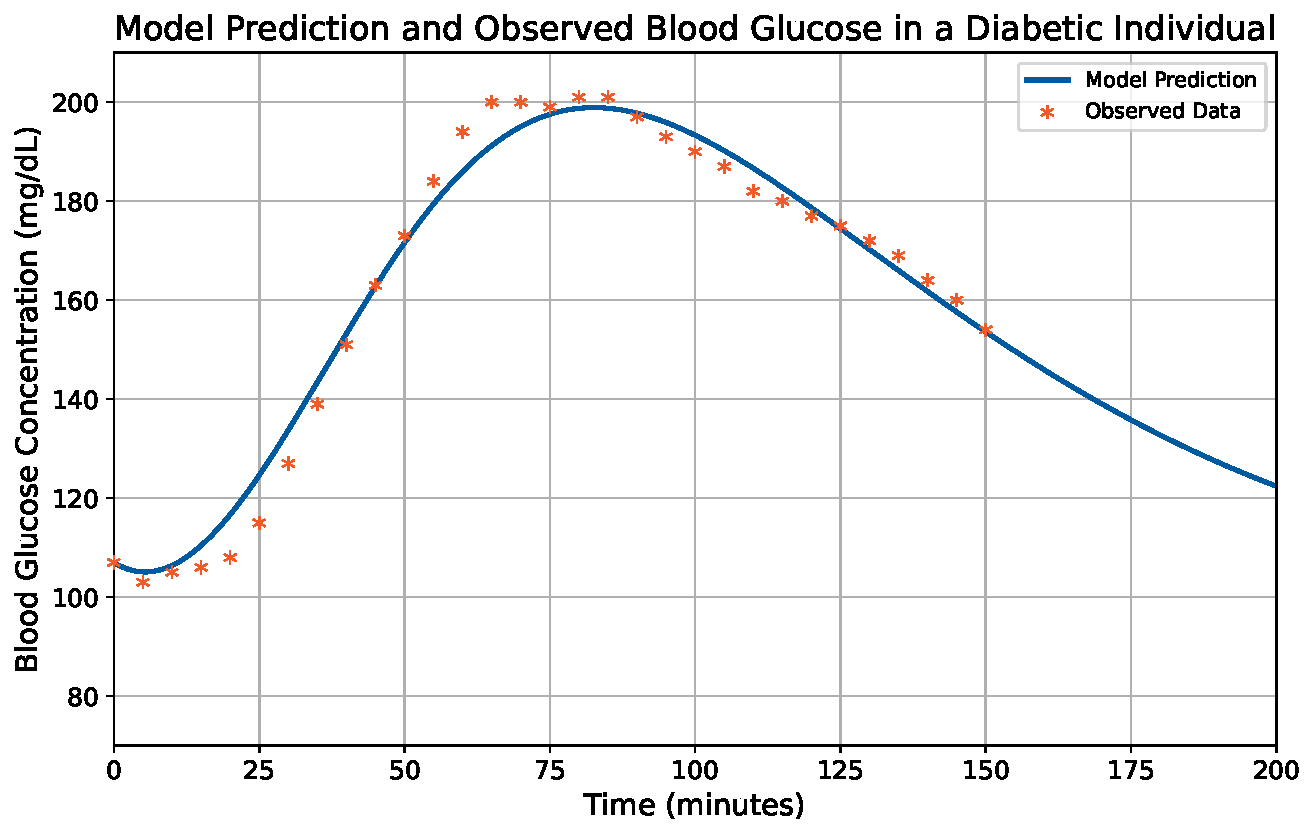
\includegraphics[width=\linewidth]{Figures/Model Prediction and Observed Blood Glucose in a Diabetic Individual.pdf}
    \end{minipage}
    \caption{Simulation of blood glucose concentration for a healthy individual (left) and a diabetic individual (right).}
\end{figure}

From Table~\ref{table: parameter}, it can be observed that the parameters representing insulin-dependent glucose uptake $\beta$ and insulin secretion in response to glucose $\mu$ are significantly lower in the type 2 diabetic individual compared to the healthy individual. This result has been widely known through many previous studies (see \cite{Ferrannini1998,Stumvoll2005,Taylor2012}). Notably, our results further suggest that the insulin-mediated inhibition of glucagon secretion $z$ is also markedly reduced in type 2 diabetic individuals. This aspect of dysregulation has received increasing attention in recent studies \cite{Ahren2009GPCRTargets,Ceriello2016GlucagonHeart,GodoyMatos2014GlucagonT2D,Gromada2018AlphaCell,UngerCherrington2012Glucagonocentric}.

%\begin{algorithm}[H]
%\caption{Parameter Estimation through Two Stages}
%\label{alg:parameter_estimation}

%\KwIn{$\{t_i\}_{i=1}^n$, $\{G_1^{\text{obs}}(t_i)\}$, 
%$\{G_2^{\text{obs}}(t_i)\}$, Model $(\ref{eq: model with no %treatment})$}

%\KwOut{Estimated parameter $\hat{p}$}

%\While{Stage 1: Initial Parameter Estimation}{
%    $\tilde{G}_2(t) \gets$ Cubic spline regression of $\{G_2^{\text{obs}}(t_i)\}$\;
    
 %   $p_N^* \gets 10^5$\;

 %   $p_m^* \gets \underset{p_m}{\arg\min}\displaystyle\sum_{i=1}^{N-1} \left(G_2^{\text{obs}}(t_{i + 1}) - \left(G_2^{\text{obs}}(t_i) + \displaystyle\int_{t_i}^{t_{i+1}} \left(\alpha_2 G_1(s) - \beta I(s) G_2(s) - \gamma G_2(s) + \eta G(s)\right) ds\right)\right)^2$;
%}

%\While{Stage 2: Refinement with $p_0 = [p_{\text{model}}^*, p_G^*, p_I^*]$}{
%   $p_0 \gets [p_m^*, p_G^*, p_I^*]$\;

%    $\hat{p} \gets 
%    \underset{p}{\arg\min}\displaystyle\sum_{i=1}^{N}\left(G_2(t_i,p) - G_2^{\text{obs}}(t_i)\right)^2$\;
%}
%\end{algorithm}

\begin{table}[H]
\centering
    \begin{tabular}{ccc}
       \hline
       \textbf{Parameter} & \textbf{Healthy person}  & \textbf{Diabetic person} \\
       \hline
       $\alpha_1$ & $5.7194 \times 10^{-3}$ & $4.2653 \times 10^{-2}$ \\
       $\alpha_2$ & $8.0769 \times 10^{-5}$ & $8.0119 \times 10^{-5}$ \\
       $\beta$    & $7.8026 \times 10^{-5}$ & $8.0004 \times 10^{-6}$ \\
       $\gamma$   & $1.2743 \times 10^{-2}$ & $1.1911 \times 10^{-2}$ \\
       $\eta$     & $1.2 \times 10^{-2}$    & $1.2 \times 10^{-2}$ \\
       $\sigma$   & $12$                    & $12$ \\
       $z$        & $1.0278 \times 10^{-3}$ & $2.2261 \times 10^{-4}$ \\
       $d$        & $8 \times 10^{-3}$      & $8 \times 10^{-3}$ \\
       $\mu$      & 12                      & 8.7410 \\
       $n$        & $3.9979 \times 10^{-2}$ & $8.0013 \times 10^{-3}$ \\
       $K$        & $160$                   & $160$ \\
       $G_0$      & $45$                    & $45$ \\
       $I_0$      & $1.5 $                  & $1.5 $ \\
       \hline
   \end{tabular}

\begin{tikzpicture}[overlay,remember picture]

\draw[thick, rounded corners](-3.5,2) rectangle (3.5,1.6);
\draw[thick, rounded corners](-3.5,2.4) rectangle (3.5,2.8);
\draw[thick, rounded corners](-3.5,3.95) rectangle (3.5,4.35);

\end{tikzpicture}

\caption{The estimated parameter values in both cases. The parameters of significant importance are enclosed in boxes.}
\label{table: parameter}
\end{table}

\section{Optimal Control Strategies}
In this section, we present two optimal control strategies to effectively regulate blood glucose levels. The first strategy focuses on optimizing both the insulin injection time and the administered insulin concentration in a discrete manner, while the second approach investigates the control of glucagon inhibition. The second strategy is motivated by the increasingly recognized central role of glucagon in blood glucose regulation, and becomes even more important in cases of severe insulin resistance \cite{gromada2007alpha,lund2014glucagon,GodoyMatos2014GlucagonT2D,haedersdal2018role,UngerCherrington2012Glucagonocentric}.

\subsection{Insulin therapy}
We now present the mathematical model describing the insulin therapy strategy with discrete insulin injections on time interval $[0,T]$. Let $t_0 = 0<t_1<\cdots<t_N<T=t_{N+1}$
be the impulsive time sequence, and let $\sigma_i$ denote the insulin dose administered at time $t_i$, for $i=1,\ldots,N$. The model reads as follows:
\begin{equation}\label{eq:insulin therapy}
\left\{
\begin{array}{l}

\left.
\begin{array}{l}
G_1'(t) = -\alpha_1 G_1, \\
G_2'(t) = \alpha_2 G_1
         - \beta IG_2
         - \gamma G_2 + \eta G,\\
G'(t)   = \sigma
         - z I G
         - d G, \\
I'(t)   = \dfrac{\mu G_2^2}{K^2 + G_2^2}
         - n I,
\end{array}
\right\}
\quad t \neq t_k, t \in [0,T], \\

\left.
\begin{array}{l}
G_1(t) = G_1(t^-), \\
G_2(t) = G_2(t^-), \\
G(t) = G(t^-), \\
I(t) = I(t^-) + \sigma_k,
\end{array}
\right\}
\quad t = t_k,

\end{array}
\right.
\end{equation}
where $k = 1,2,\ldots,N$.

Let 
\[
T = \{\tau = (t_1,\ldots,t_N) \in \mathbb{R}^N : a_i \le t_i \le b_i,\; i=1,\ldots,N\}
\]
and
\[
D = \{\delta = (\sigma_1,\ldots,\sigma_N) \in \mathbb{R}^N : u_i \le \sigma_i \le v_i,\; i=1,\ldots,N\},
\]
where \(a_i,b_i \in [0,T]\) with \(b_i \le a_{i+1}\) for \(i=1,\ldots,N-1\), and \(u_i,v_i>0\) for all \(i=1,\ldots,N\). To ensure that blood glucose levels remain within the normal physiological range $[T_1, T_2]$ while avoiding excessive insulin administration, which may lead to hyperinsulinemia-related metabolic imbalance and other adverse physiological effects, we define the following objective function
\begin{equation}\label{Obj 1}
    \underset{\tau \in T, \delta \in D}{\min} J(\tau, \delta) = \omega\displaystyle\sum_{i=1}^{N} \sigma_i^2 + \int\limits_0^T (G_2(s) - T_1)(G_2(s)-T_2)\, ds,
\end{equation}
where $T, \omega > 0$ and $T_2 > T_1 > 0$.

To establish the existence of an optimal control $(\tau^*,\delta^*)$ for problem \eqref{eq:insulin therapy}-\eqref{Obj 1}, we employ the stacking argumentation. This method is widely used in the analysis of impulsive optimal control problems, where the original impulsive trajectory is represented as an equivalent continuous system defined on stacked subintervals. Stacking means that all subintervals from the impulsive trajectory are treated as if they evolve
simultaneously in the transformed problem \cite{Bohme2017,liu1998statejumps}.

We transform system \eqref{eq:insulin therapy} defined on each interval $[t_{i-1},t_i)$ into an equivalent system on $[0,1)$. For $t \in [t_{i-1}, t_i)$, let $t = t_{i-1} + (t_i-t_{i-1})s$, where $s \in [0,1)$. For each state variable $x \in \{G_1, G_2, G, I\}$, we define 
\begin{equation*}
    y_{(i)}(s) = x(t_{i-1}+(t_i-t_{i-1})s).
\end{equation*}
Let $\zeta_i = t_i - t_{i-1}, i =1,2,...,N+1$. Then $y_{(i)}'(s) = \zeta_i x'(t(s))$ and system \eqref{eq:insulin therapy} is transformed into the following $N+1$ subsystems:

\begin{equation}\label{eq:insulin therapy transform}
\begin{cases}
G_{1(i)}'(s) = -\alpha_1\zeta_i G_{1(i)}, \\
G_{2(i)}'(s) = \alpha_2\zeta_i G_{1(i)}
         - \beta\zeta_i I_{(i)}G_{2(i)}
         - \gamma\zeta_i G_{2(i)}
         + \eta\zeta_i G_{(i)},\\
G_{(i)}'(s) = \sigma\zeta_i
         - z\zeta_i I_{(i)} G_{(i)}
         - d\zeta_i G_{(i)}, \\
I_{(i)}'(s) = \frac{\mu\zeta_i G_{2(i)}^2}
         {K^2 + G_{2(i)}^2}
         - n\zeta_i I_{(i)},\\
\end{cases}
\end{equation}
where $s \in [0,1), i = 1,2,\ldots,N+1$, and 
\begin{equation}\label{eq:insulin therapy transform boundary}
\begin{cases}
G_{1(i+1)}(0) = G_{1(i)}(1), \\
G_{2(i+1)}(0) = G_{2(i)}(1), \\
G_{(i+1)}(0) = G_{(i)}(1), \\
I_{(i+1)}(0) = I_{(i)}(1) + \sigma_i,
\end{cases}
\end{equation}
where $i = 1,2,\ldots,N$. 

It is clear that $\zeta_1+\zeta_2+\ldots+\zeta_N+\zeta_{N+1} = T$. Let 
\[
T' = \{\zeta = (\zeta_1,\ldots,\zeta_N) \in \mathbb{R}^{N}: a_1 \le \zeta_1 \le b_1, a_{i}-b_{i-1} \le \zeta_i \le b_{i}-a_{i-1} \text{ for } i = 2,3,\ldots,N \}.
\]
The objective function \eqref{Obj 1} is transformed into
\begin{equation}\label{Obj 1 transform}
    \underset{\zeta \in T', \delta \in D}{\min} J'(\zeta, \delta) = \omega\displaystyle\sum_{i=1}^{N} \sigma_i^2 + \displaystyle\sum_{i=1}^N \int\limits_0^1 (G_2(s) - T_1)(G_2(s)-T_2)\, ds,
\end{equation}
where $T, \omega > 0$ and $T_2 > T_1 > 0$.

\begin{theorem}
    There exists an optimal control $(\tau^*,\delta^*) \in T\times D$ for problem \eqref{eq:insulin therapy}-\eqref{Obj 1} for every initial state in $\mathbb{R}^4_{> 0}$.
\end{theorem}

\begin{proof}
    
\end{proof}

Necessary optimality conditions for optimal control problems with state jumps have been extensively studied in the literature (see \cite{hu2005optimization,liu2023impulsive,liu1998statejumps}). To derive necessary conditions for optimal control for problem \eqref{eq:insulin therapy}-\eqref{Obj 1}, we apply Theorem $1$ from \cite{liu2023impulsive} as follows: 
\begin{theorem}
    Considering the impulsive system \eqref{eq:insulin therapy} and the objective function $J(\tau,\delta)$ in \eqref{Obj 1}. If $(\tau^*,\delta^*)$ is optimal for problem \eqref{eq:insulin therapy}-\eqref{Obj 1}, then there exists a piecewise differentiable adjoint variable  $\lambda(t) = (\lambda_1(t),\lambda_2(t),\lambda_3(t),\lambda_4(t))^\top$ satisfies:
    \begin{itemize}
        \item Euler-Lagrange equation. 
        \[
        \begin{cases}
            \lambda_1'(t) &= \alpha_1\lambda_1 - \alpha_2\lambda_2, \\
            \lambda_2'(t) &= T_1+T_2-2G_2 + (\beta I + \gamma)\lambda_2 - \dfrac{2\mu K^2G_2}{(K^2+G_2^2)^2}\lambda_4, \\
            \lambda_3'(t) &= -\eta\lambda_2 + (zI+d)\lambda_3, \\
            \lambda_4'(t) &= \beta G_2\lambda_2 + zG\lambda_3 + n\lambda_4,
        \end{cases}
        \]
        for all $t \neq t_i^*, i = 1,2,...,N$.
        \item Boundary conditions.
        \[
        \begin{cases}
            \lambda(t_i^{*-}) &= \lambda(t_i^{*+}), \\
            \lambda(T) &= 0,
        \end{cases}
        \]
        for all $i = 1,2,...,N$.
        \item Optimality conditions.
        \[
        \begin{cases}
        \begin{aligned}
            \dfrac{\partial J}{\partial \sigma_i}(\tau^*,\delta^*) &= 2\omega\sigma_i^* + \lambda_4(t_i^{*+}) &= 0, \\
            \dfrac{\partial J}{\partial t_i}(\tau^*, \delta^*) &= H(t_i^{*-}) - H(t_i^{*+}) &= 0,
        \end{aligned}
        \end{cases}
        \]
        for all $i = 1,2,...,N$, where Hamilton function 
        \begin{align*}
            H(G_1,G_2,G,I,\lambda) = &\text{ }G_2^2 - (T_1 + T_2)G_2 + T_1T_2 - \alpha G_1\lambda_1 + (\alpha_2G_1-\beta I G_2 - \gamma G_2 + \eta G)\lambda_2 \\
            &+ (\sigma - zIG -dG)\lambda_3 + \bigg(\dfrac{\mu G_2^2}{K^2 + G_2^2} - nI\bigg)\lambda_4.
        \end{align*}
    \end{itemize}
\end{theorem}

\begin{proof}
    
\end{proof}

\begin{algorithm}[H]
\caption{Gradient-based optimization of control variables}
\SetKwInOut{Input}{Input}
\SetKwInOut{Output}{Output}
\SetKw{RETURN}{return}

\Input{Initial control $\tau^{(0)},\delta^{(0)}, x_0 \in \mathbb{R}^n$}
\Output{Optimal control variables $\tau, \delta$}

$k \gets 0$\;

\While{$k < k_{\max} \textbf{ and } \left(\left\| \frac{\partial J}{\partial \tau} \right\| > \varepsilon_1 \ \textbf{or} \ \left\| \frac{\partial J}{\partial \delta} \right\| > \varepsilon_2\right)$}{
    Solve the state system forward in time to obtain $x(t),\ t \in [0, T]$\;
    
    Solve the costate system backward in time to obtain $\lambda(t),\ t \in [0, T]$\;
    
    Compute the gradients:
    \[
    \dfrac{\partial J}{\partial \tau^{(k)}}
    \gets
    \begin{bmatrix}
    \dfrac{\partial J}{\partial t_1^{(k)}} & \cdots & \dfrac{\partial J}{\partial t_N^{(k)}}
    \end{bmatrix}^T,
    \quad
    \dfrac{\partial J}{\partial \delta^{(k)}}
    \gets
    \begin{bmatrix}
    \dfrac{\partial J}{\partial \sigma_1^{(k)}} & \cdots & \dfrac{\partial J}{\partial \sigma_N^{(k)}}
    \end{bmatrix}^T ;
    \]
    
    Update the control variables:
    \[
    \tau^{(k+1)} \gets \tau^{(k)} - \alpha \dfrac{\partial J}{\partial \tau^{(k)}}, 
    \quad
    \delta^{(k+1)} \gets \delta^{(k)} - \beta \dfrac{\partial J}{\partial \delta^{(k)}} ;
    \]
    $k\gets k + 1$ \;
}
\RETURN $\tau^{(k)}, \delta^{(k)}$ \;
\end{algorithm}

\subsection{Glucagon inhibition}
\begin{equation}\label{eq:glucagon inhibition}
    \begin{cases}
        G_1'(t) &= -\alpha_1 G_1, \\
        G_2'(t) &= \alpha_2 G_1
                 - \beta IG_2
                 - \gamma G_2 + \eta\, G,\\
        G'(t)   &= u(t)\sigma
                 - z\, I\, G
                 - d\, G, \\
        I'(t)   &= \dfrac{\mu G_2^2}{K^2 + G_2^2}
                 - n\, I,
    \end{cases}
\end{equation}

Let $U = \{u \in L^\infty(0,T): 0 \le u(t) \le 1\}$.

Objective function:
\[
\underset{u \in U}{\min} J[u(\cdot)] = \int_0^T (G_2(s) - T_1)(G_2(s)-T_2) + u^2(s)\, ds,
\]

Define the Hamiltonian function as
\[
\begin{aligned}
H &= (G_2 - T_1)(G_2 - T_2) + u^2 + \lambda_1(-\alpha_1 G_1) + \lambda_2\big(\alpha_2 G_1 - \beta I G_2 - \gamma G_2 + \eta G\big) \\
& \quad + \lambda_3\big(u\sigma - z I G - d G\big) + \lambda_4\left(\frac{\mu G_2^2}{K^2 + G_2^2} - n I\right).
\end{aligned}
\]

According to Pontryagin's Maximum Principle, there exist adjoint variables \(\lambda_1(t), \lambda_2(t), \lambda_3(t), \lambda_4(t)\) satisfying
\[
\begin{cases}
\dot{\lambda}_1 
= \alpha_1 \lambda_1 - \alpha_2 \lambda_2, \\

\dot{\lambda}_2 
= T_1 + T_2 - 2G_2
+ (\beta I + \gamma)\lambda_2
- \dfrac{2\mu K^2 G_2}{(K^2 + G_2^2)^2}\lambda_4, \\

\dot{\lambda}_3 
= -\eta \lambda_2 + (zI + d)\lambda_3, \\

\dot{\lambda}_4 
= \beta G_2 \lambda_2 + zG \lambda_3 + n\lambda_4, \\
\lambda_i(T) = 0, \quad i=1,2,3,4.
\end{cases}
\]

Since the Hamiltonian is strictly convex with respect to \(u\), the optimal control is characterized by the first-order condition
\[
\frac{\partial H}{\partial u} = 2u + \sigma \lambda_3 = 0.
\]
Taking into account the control constraints \(0 \le u(t) \le 1\), the optimal control is obtained by projecting the stationary point onto the admissible set, that is,
\[
u^*(t) = \min\left(1, \max\left(0, -\frac{\sigma\lambda_3(t)}{2}\right)\right).
\]

\begin{algorithm}
    \caption{FBSM}
    \SetKwInOut{Input}{Input}
    \SetKwInOut{Output}{Output}
    \SetKw{RETURN}{return}

    \Input{Initial control $u^{(0)} (t)$, state $x_0$, tolerance $\varepsilon$, max iteration $k_{\max}$, relaxation $\alpha \in (0, 1]$}
    \Output{Optimal control $u^*(t)$}
    $k \gets 0$ \;
    \While{$\left\|u^{(k+1)}-u^{(k)}\right\| > \varepsilon$ \textbf{or} $k < k_{\max}$}{
        Solve the state trajectory $x(t)$, $t\in [0,T]$ forward in time\;

        Solve the costate trajectory $\lambda(t)$, $t \in [0,T]$ backward in time\;
        
        Compute optimal control:
        \[
            \tilde{u}(t) \gets \min\left(1, \max\left(0, -\frac{\lambda_3(t)\sigma}{2} \right)\right) ;
        \]
        
        Update control:
        \[
            u^{(k+1)}(t)
            \gets
            (1-\alpha)u^{(k)}(t)
            +
            \alpha \tilde{u}(t) ;
        \]
        $k \gets k + 1$;
    }
    \RETURN $u^{(k)}(t)$\;
\end{algorithm}

\section{Discussion}

\bibliographystyle{plain}  
\bibliography{ref}   

\section*{Appendices}

\end{document}